\documentclass[12pt,a4paper, twosite]{article}
\usepackage[utf8]{inputenc}
\usepackage[T1]{fontenc}
\usepackage{graphicx}
\usepackage{grffile}
\usepackage{longtable}
\usepackage{wrapfig}
\usepackage{rotating}
\usepackage[normalem]{ulem}
\usepackage{amsmath}
\usepackage{textcomp}
\usepackage{amssymb}
\usepackage{capt-of}
\usepackage{hyperref}
\usepackage[left=2.00cm, right=2.50cm, top=2.50cm, bottom=2.00cm]{geometry}
\usepackage{fancyhdr}
\usepackage[spanish]{babel}
\fancyhead[RO,LE]{\thepage}
\fancyhead[LO]{\emph{\uppercase{\leftmark}}}
\fancyfoot{}
\renewcommand{\headrulewidth}{1.0pt}
\pagestyle{fancy}
\date{\today}
\title{IEEE-830}
\hypersetup{
	pdfborder={0 0 0},
	pdfauthor={fasdas ads d},
	pdftitle={IEEE-830},
	pdfkeywords={hola},
	pdfsubject={hola mundo},
%	pdfcreator={Emacs 26.2 (Org mode 9.1.9)}, 
	pdflang={Spanish}}


\begin{document}
	\begin{titlepage}
		\maketitle
		
	\end{titlepage}

\section*{Historial de cambios  }
crear tabla de el versionado de los cambios 

\newpage
	\tableofcontents	
\newpage
	\section{Introducción}
	\label{sec:org60390fa}



	
	\subsection{Propósito}
	\label{sec:org434c3ef}
	Este documento presenta una especificación de requerimientos de software para unsistema de  posicionamiento de antena. Este dispositivo generalmente se conoce como rotador. 
	 
	Esta dirigido a técnicos, profesionales y operarios que intervengan en los sistemas de apuntamiento que posee el IAR.   

	
	
	\subsection{Ámbito del sistema}
	\label{sec:org12e44a1}
	Este sistema, se desarrolla como un subsistema del interferómetro MIA(https://www.iar.unlp.edu.ar/slider/observatorio/), y el proyecto de construcción de estaciones terrenas. Se utilizar para realizar el apuntamiento de radiofuentes, y el seguimiento de satelites en forma automática.  El nombre del sistema rotador sera ROT\_IAR. Adicionalmente, tiene espectativas de escalar, y realizar una producción en serie. 
	
	
	\subsection{Definiciones, Acrónimos y Abreviaturas}
	\label{sec:orgb158e36}
	
	ver los acrónimos al terminar el documento 
	
	
	\subsection{Referencias}
	\label{sec:org62711e0}
	ver tesis, y plan de trabajo ! 
	
	\subsection{Visión general del documento}
	\label{sec:orgdaca22c}
	
	Este documento se realiza siguiendo el estándar IEEE Std. 830-1998
	
	
	\section{Descripción general del documento}
	\label{sec:orgc1c4017}
	
	\subsection{Perspectiva del producto}
	\label{sec:org24980a8}
%	El proyecto aquí especificado es independiente de otros sistemas y no tiene relación con otros productos
	El software es parte de un sistema mayor, denominado interferómetro MIA y estaciones terrenas. Este sistema de apuntamiento, se adicionara al sistema mecánico de la antena que esta en fase de construcción. Este sistema, realizará el apuntamiento de antena, y este según el proyecto(MIA o estaciones terrenas) es automático o manual. El diagrama en bloques del sistema se muestra en la figura \ref{fig:diagramaBloques}. 
	
	 El presente documento describe los requerimientos de software del bloque single board computer, y las interfaces del sistema que se observa en la figura  \ref{fig:diagramaBloques}. 
	\begin{figure}[h!]
		\centering
		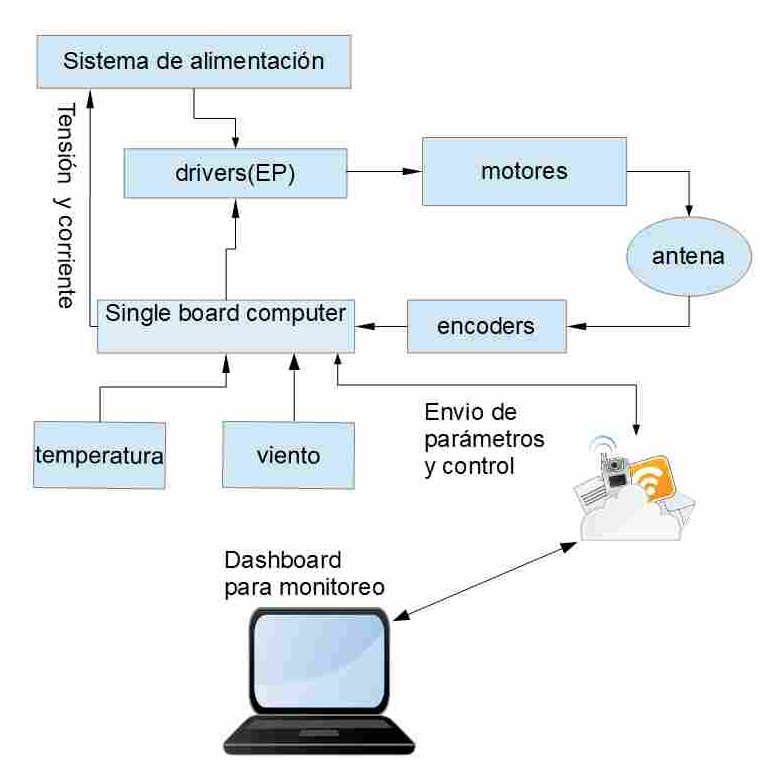
\includegraphics[scale=0.5]{bloquesInt.jpg}
		\caption{Diagrama en bloques del sistema}
		\label{fig:diagramaBloques}
	\end{figure}
	\subsection{Funciones del producto}
	\label{sec:orgaf51da6}
	\begin{enumerate}
		\item control de posición
		\item Servidor web embebido 
		\item Compatible con el software Gpredict y Stellarium, y scripts de antenas principales 
		\item Reinicio del en forma remota  
		\item Interrupción de operación en caso de condiciones climáticas adversas. 
		\item información de la operación y estado actual del sistema(tracking, untracked, y cenit). 
	\end{enumerate}
	
	\subsection{Características de los usuarios}
	\label{sec:orga40b0ee}
	Los usuarios serán técnicos, operarios y profesionales con conocimiento y experiencia en los sistemas de apuntamiento y manejo de rotadores. 
	\subsection{Restricciones}
	\label{sec:org5ca5790}
	
	
	\begin{itemize}
		
		\item Lenguaje python3 por cuestiones de compatibilidad de scripts de manejo principal de las antenas.
		\item El software debe estar bajo control de versiones.  
%		\item  se debe realizar un informe de avance por cada requerimiento que se cumple 
	\end{itemize}
	
	
	\subsection{Suposiciones y dependencias}
	\label{sec:org0ae23fe}
	Se supone que se cuenta con los scripts del manejo de las antenas principales 
	
	Se cuenta con los encoders y motores seleccionados. 
	
	
	\subsection{Requisitos futuros}
	\label{sec:org33cfcdb}
	El sistema posea control de velocidad 
	El diseño electrónico escalable, y realizable en una cadena de producción.  
	El sistema debe poseer autocalibración en base al sol o la luna(esto dependerá del horario en que se realice la autocalibración) 
	
	
	
	
	\section{Requisitos específicos}
	\label{sec:org40573d1}
	
	
	\subsection{Interfaces externas}
	\label{sec:orgfd5391f}
	\begin{itemize}
		\item El sistema se comunicara con una red local mediante cable ethernet con conector RJ45
		\item El sistema se conecta con un sensor de temperatura DHT11 mediante onewire. 
		\item El sistema se conecta con los drivers de los motores mediante puertos que posean salida PWM. 
		\item Los encoders serán conectados en un puerto analógico digital. 
		\item El sistema de medición del viento se realizará con un anemómetro, y se conectará a un puerto analógico digital
		\item Se realizará un PCB que se acople al single board computer mecánicamente con borneras, donde se indique mediante serigrafia donde se conecta. Esta serigrafia será: 
		\begin{itemize}
			\item EP1: motor de azimuth 
			\item EP2: motor de altura
			\item ENC1: encoder de azimuth 
			\item ENC2: encoder de altura 
			\item VTO: anemómetro 
			
		\end{itemize} 
		
	\end{itemize}
	
	\subsection{Funciones}
	\label{sec:org307bb59}
	\subsection{Control de posición}
	\begin{enumerate}
		\item El sistema debe   
		\item El control debe realizarse mediante un control on/off. 
	\end{enumerate}
	
	
	
	
	\subsection{Requisitos de rendimiento}
	\label{sec:org94bc543}
	
	Se detallarán los requisitos relacionados con la carga que se espera
	tenga que soportar el sistema. Por ejemplo, el número de terminales,
	el número esperado de usuarios simultaneamente conectados, número de
	transacciones por segundo que deberá soportar el sistema, etc.
	También, si es necesario, se especificarpán los requisitos de
	datos, es decir, aquellos requisitos que afecten a la información
	que se guardará en la base de datos. Por ejemplo, la frecuencia de
	uso, las capacidades de acceso y la cantidad de registros que se
	espera almacenar (decenas, cientos, miles o millones).
	
	
	\subsection{Restricciones de diseño}
	\label{sec:org49fe900}
	
	
	Todo aquello que restrinja las decisiones relativas al diseño de la
	aplicación: Restricciones de otros estándares, limitaciones del
	hardware, etc.
	
	
	\subsection{Atributos del sistema}
	\label{sec:orgd0babc0}
	
	Se detallarán los atributos de calidad (las "ilities") del
	sistema. Fiablidad, manteniblidad, portabilidad, y muy importante,
	la seguridad. Deberá especificarse qué tipos de usuarios están
	autorizados, o no, a realizar ciertas tareas, y cómo se
	implementarán los mecanismos de seguridad (por ejemplo, por medio de
	un \emph{login} y una \emph{password}).
	
	
	\subsection{Otros requisitos}
	\label{sec:org31d2978}
	
	Cualquier otro requisito que no encaje en otra sección.
	
	\newpage
	
	
	\section{Apéndices}
	\label{sec:org75cea03}
	
	Puede contener todo tipo de información relevante para la ERS pero
	que, propiamente, no forme parte de la ERS. Por ejemplo:
	
	\begin{enumerate}
		\item Formatos de entrada/salida de datos, por pantalla o en listados.
		
		\item Resultados de análisis de costes.
		
		\item Restricciones acerca del lenguaje de programación.
	\end{enumerate}
\end{document}